\chapter{Experimentos}\label{sec:experiments}
%======================================================================================
No presente trabalho, nos concentramos no objetivo proposto descrito na Seção~\ref{sec:objetivo}.

\section {Procedimento}
Primeiramente, filmamos algumas esculturas utilizando a câmera de um {\it smartphone} convencional na resolução de 1920x1080 pixels. Esta filmagem foi realizada varrendo toda (ou maioria) da superfície da escultura em 360$^{\circ}$ com o intuito de ter toda a escultura reconstruída \ref{fig:procedimentoscan}.
Após isso, fizemos mais alguns vídeos, pegando alguns pontos que possuíam mais detalhes e que, com uma única varredura, não era capaz de reproduzir uma boa reconstrução.

\begin{figure}[!h]
	\centering
	%   \includegraphics[width=1.0\linewidth]{figs/3d-curve-sketch/system-diagram.eps}
	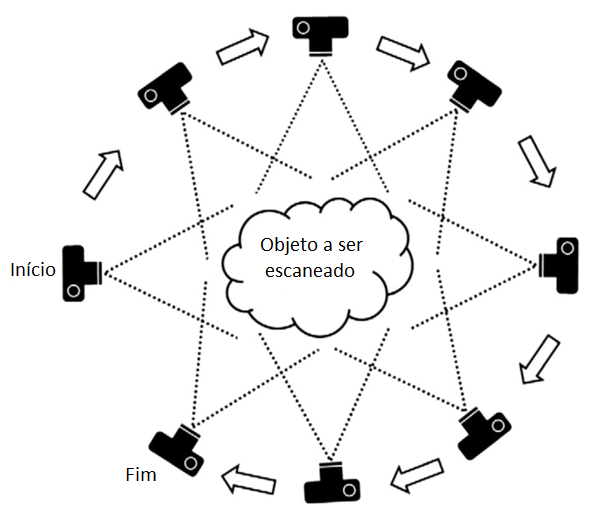
\includegraphics[width=0.5\linewidth]{figs/procedimentoscan.png}
	\caption{%
	Exemplo de como foi realizada a varredura da escultura
	%\cite{Cui:Theobalt:etal:PAMI2013,Pajdla:etal:ICCV2011}.
	}\label{fig:procedimentoscan}
\end{figure}

Com este material, foram feitos "cortes" em determinados {\it frames} do vídeo, com atenção para não cortar em {\it frames} muito juntos, pois aumentaria o número de correspondências ambíguas entre as imagens e com isso, o processamento da reconstrução demoraria mais. E não usar {\it frames} muito distantes, o que ocorreria o inverso, com menos correspondências, ficariam buracos na reconstrução. Como descrito na Seção \ref{sec:mve}.
Com isso em mente, foram reconstruídas duas esculturas: uma com um único vídeo, usando o VisualSfM, totalizando 200 imagens e outra com dois vídeos, com o MVE, com dois vídeos, que, ao cortá-los, totalizou cerca de 280 imagens.

%COLOCAR PROCEDIMENTO DO MVE E VISUALSFM AQUI%

Além de esculturas ao ar livre, fizemos alguns testes em ambiente fechado, dentro de uma casa, por exemplo. Foi utilizado um objeto feito de cabaça (casca de abóbora) na qual possui uma superfície propícia para uma reconstrução (Seção \ref{sec:laser}, sobre superfícies Lambertianas). 

Com o procedimento descrito anteriormente, a partir dos vídeos feitos, obtemos um total de 200 imagens em um vídeo superficial e mais 24 imagens mais detalhadas do objeto, ambos numa resolução de 1080x1920 pixels. E, para um mesmo conjunto de imagens, rodamos tanto o VisualSfM quanto o MVE.

\subsection{Resultados da reconstrução do objeto com o VisualSfM}
Seguindo o passo-a-passo de reconstrução do {\it software}, obtemos os seguintes resultados:

\begin{table}
\caption{Tempos obtidos da reconstrução do objeto usando o VisualSfM}
\label{tab:temposSfM}
\begin{tabular}{|l|p{4.7cm}|}
\hline
Procedimento & Tempo \\ \hline
Carregamento de imagens & 50 segundos \\ \hline
Calcular pares correspondentes de {\it features} & 159 segundos \\ \hline
Gerar a reconstrução esparsa do modelo & 135 segundos \\ \hline
Gerar a reconstrução densa do modelo & 1416 segundos \\ \hline
\end{tabular}
\end{table}

A figura \ref{fig:reconstrucaoEsparsaVisualSFM} mostra, o resultado da reconstrução esparsa do algoritmo PBA. Não é tão nítida como na figura \ref{fig:reconstrucaoDensaVisualSFM}, a quantidade de ruídos, provenientes de outros objetos (o VisualSfM só identifica objetos estáticos) presentes na cena, e não é possível limpar a malha no próprio {\it software}, somente por meio de programas externos.

\begin{figure}[!h]
	\centering
	%   \includegraphics[width=1.0\linewidth]{figs/3d-curve-sketch/system-diagram.eps}
	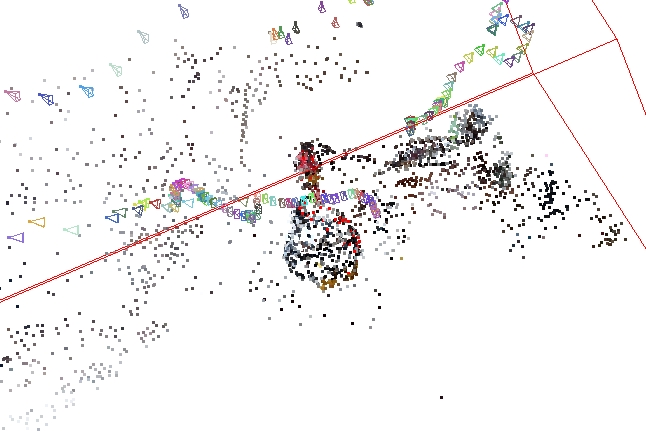
\includegraphics[width=0.5\linewidth]{figs/galinhasparsa.jpg}
	\caption{%
	Reconstrução esparsa do objeto no VisualSfM
	%\cite{Cui:Theobalt:etal:PAMI2013,Pajdla:etal:ICCV2011}.
	}\label{fig:reconstrucaoEsparsaVisualSFM}
\end{figure}

\begin{figure}[!h]
	\centering
	%   \includegraphics[width=1.0\linewidth]{figs/3d-curve-sketch/system-diagram.eps}
	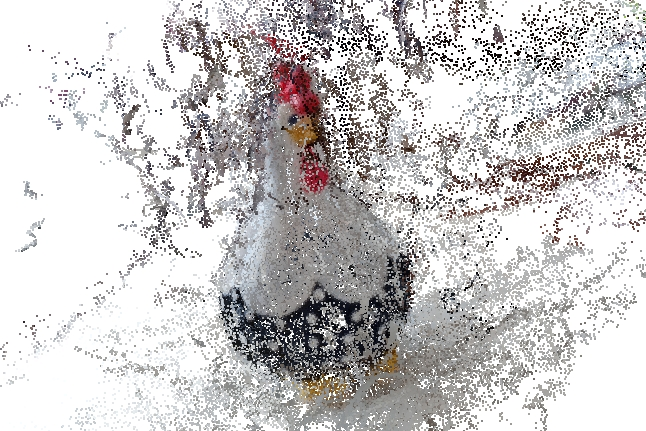
\includegraphics[width=0.5\linewidth]{figs/galinhadense.jpg}
	\caption{%
	Reconstrução densa do objeto no VisualSfM
	%\cite{Cui:Theobalt:etal:PAMI2013,Pajdla:etal:ICCV2011}.
	}\label{fig:reconstrucaoDensaVisualSFM}
\end{figure}

Fizemos uma outra reconstrução, utilizando os dois vídeos (gerando 224 imagens), caso fosse usado um conjunto maior, o programa parava de funcionar por falta de memória, mesmo após ajustar parâmetros (como o número de vizinhos, número de {\it cores} do processador, {\it level} do PMVS usado, entre outros) para melhorar esse problema. Com isso em mente, conseguimos os seguintes resultados:

\begin{table}
\caption{Tempos obtidos da reconstrução do objeto, com 224 imagens usando o VisualSfM}
\label{tab:temposSfM224}
\begin{tabular}{|l|p{4.7cm}|}
\hline
Procedimento & Tempo \\ \hline
Carregamento de imagens & 60 segundos \\ \hline
Calcular pares correspondentes de {\it features} & 200 segundos \\ \hline
Gerar a reconstrução esparsa do modelo & 162 segundos \\ \hline
Gerar a reconstrução densa do modelo & 1920 segundos \\ \hline
\end{tabular}
\end{table}

Percebemos que não foi tão proveitoso (qualitativamente) usar mais imagens neste caso, inclusive o algoritmo perdeu a referência do objeto e gerou um segundo modelo na reconstruçãoe esparsa \ref{fig:reconstrucaoEsparsaVisualSFM224}, e consequentemente, na reconstrução densa \ref{fig:reconstrucaoDensaVisualSFM2241} e \ref{fig:reconstrucaoDensaVisualSFM2242}. O que gerou uma cerca incoerência na reconstrução.

\begin{figure}[!h]
	\centering
	%   \includegraphics[width=1.0\linewidth]{figs/3d-curve-sketch/system-diagram.eps}
	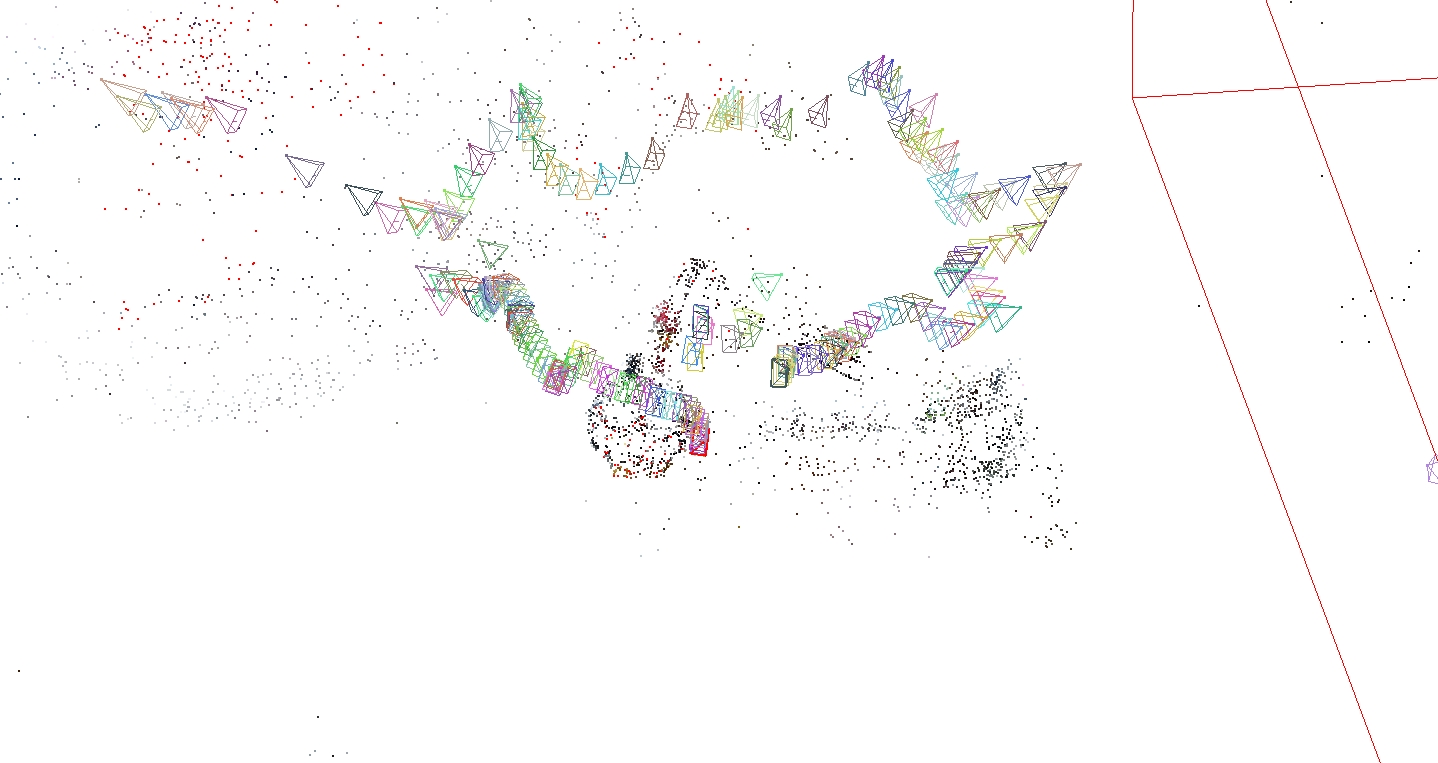
\includegraphics[width=0.5\linewidth]{figs/perto_longe_esparsa.jpg}
	\caption{%
	Reconstrução esparsa do objeto com 224 imagens no VisualSfM
	%\cite{Cui:Theobalt:etal:PAMI2013,Pajdla:etal:ICCV2011}.
	}\label{fig:reconstrucaoEsparsaVisualSFM}
\end{figure}

\begin{figure}[!h]
	\centering
	%   \includegraphics[width=1.0\linewidth]{figs/3d-curve-sketch/system-diagram.eps}
	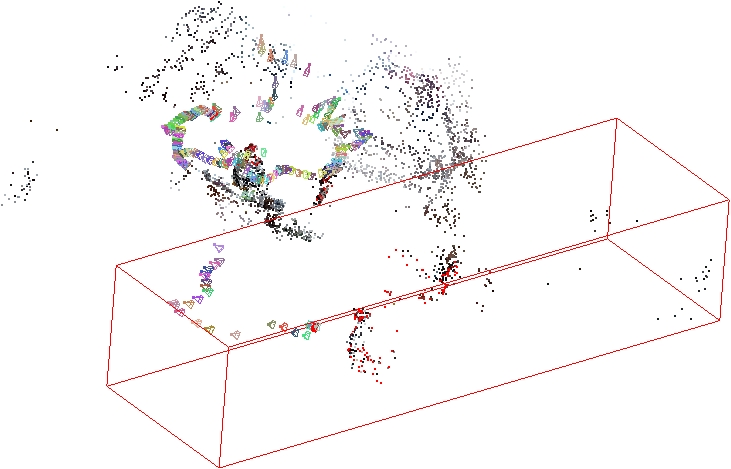
\includegraphics[width=0.5\linewidth]{figs/perto_longe_esparsa_2.jpg}
	\caption{%
	Foi gerado dois modelos esparsos do objeto a partir do conjunto inicial de 224 imagens, provavelmente, proveniente da falta de parâmetros da câmera
	%\cite{Cui:Theobalt:etal:PAMI2013,Pajdla:etal:ICCV2011}.
	}\label{fig:reconstrucaoEsparsaVisualSFM224}
\end{figure}

\begin{figure}[!h]
	\centering
	%   \includegraphics[width=1.0\linewidth]{figs/3d-curve-sketch/system-diagram.eps}
	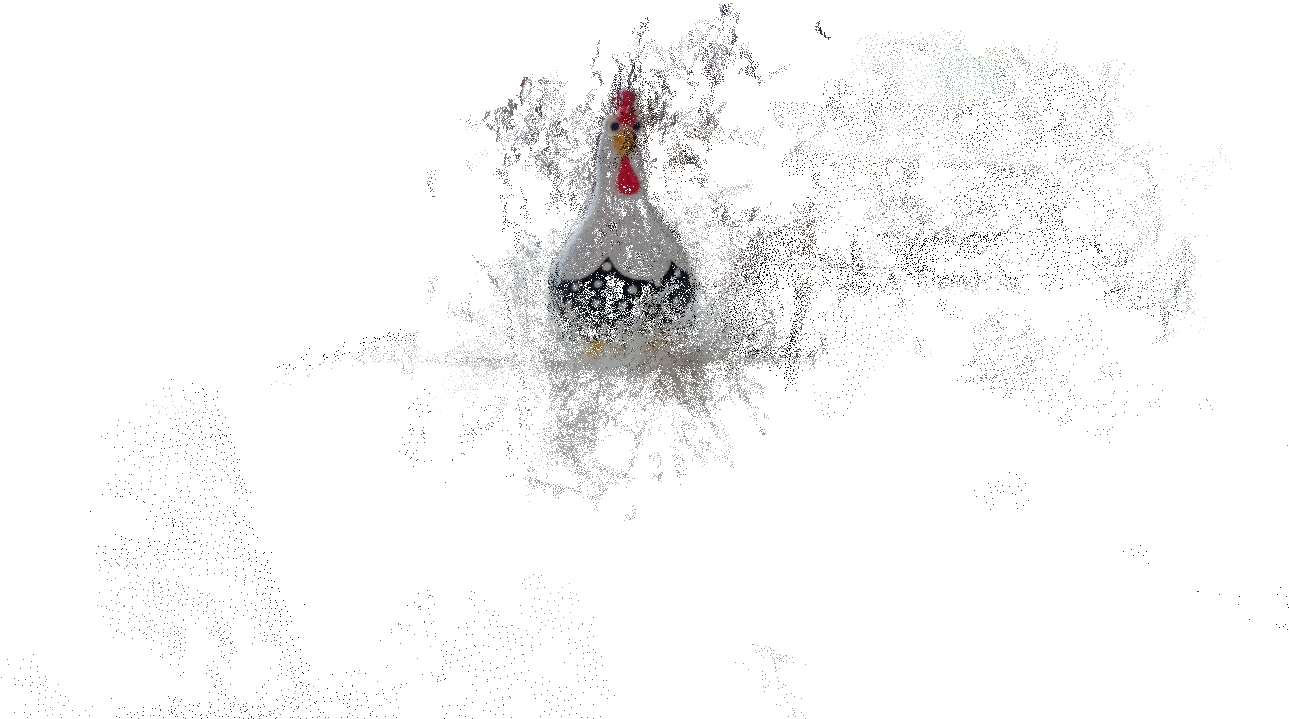
\includegraphics[width=0.5\linewidth]{figs/galinhadense224.jpg}
	\caption{%
	Reconstrução do primeiro modelo do objeto no VisualSfM com 224 imagens
	%\cite{Cui:Theobalt:etal:PAMI2013,Pajdla:etal:ICCV2011}.
	}\label{fig:reconstrucaoDensaVisualSFM2241}
\end{figure}

\begin{figure}[!h]
	\centering
	%   \includegraphics[width=1.0\linewidth]{figs/3d-curve-sketch/system-diagram.eps}
	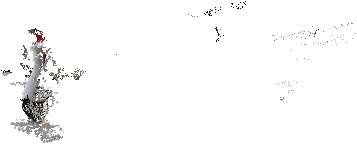
\includegraphics[width=0.5\linewidth]{figs/galinhavisualsfm224.jpg}
	\caption{%
	Reconstrução do segundo modelo do objeto no VisualSfM com 224 imagens
	%\cite{Cui:Theobalt:etal:PAMI2013,Pajdla:etal:ICCV2011}.
	}\label{fig:reconstrucaoDensaVisualSFM2242}
\end{figure}

\subsection{Resultados da reconstrução do objeto com o MVE}

Com a interface gráfica (UMVE), criamos uma nova cena e inserimos, primeiramente, as 200 fotos do objeto. Em seguida, utilizando as linhas de comando do MVE, fizemos o procedimento padrão de reconstrução do {\it software}. E, obtivemos os seguintes resultados:

\begin{figure}[!h]
	\centering
	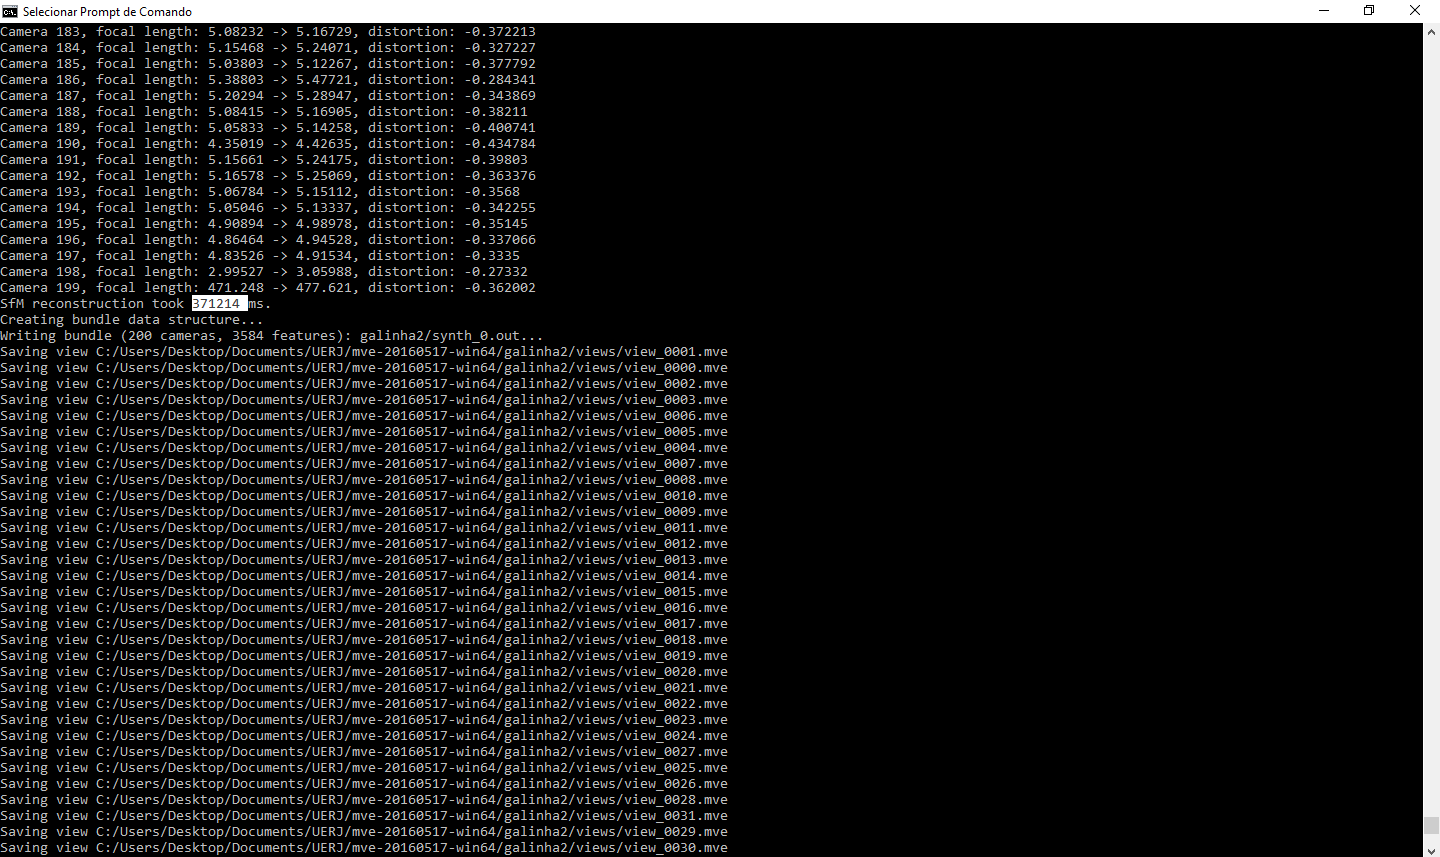
\includegraphics[width=0.5\linewidth]{figs/galinhalongesfmreconmve.png}
	\caption{%
	Tempo gasto da etapa {\it sfmrecon} do MVE
	}\label{fig:sfmrecon1}
\end{figure}

\begin{figure}[!h]
	\centering
	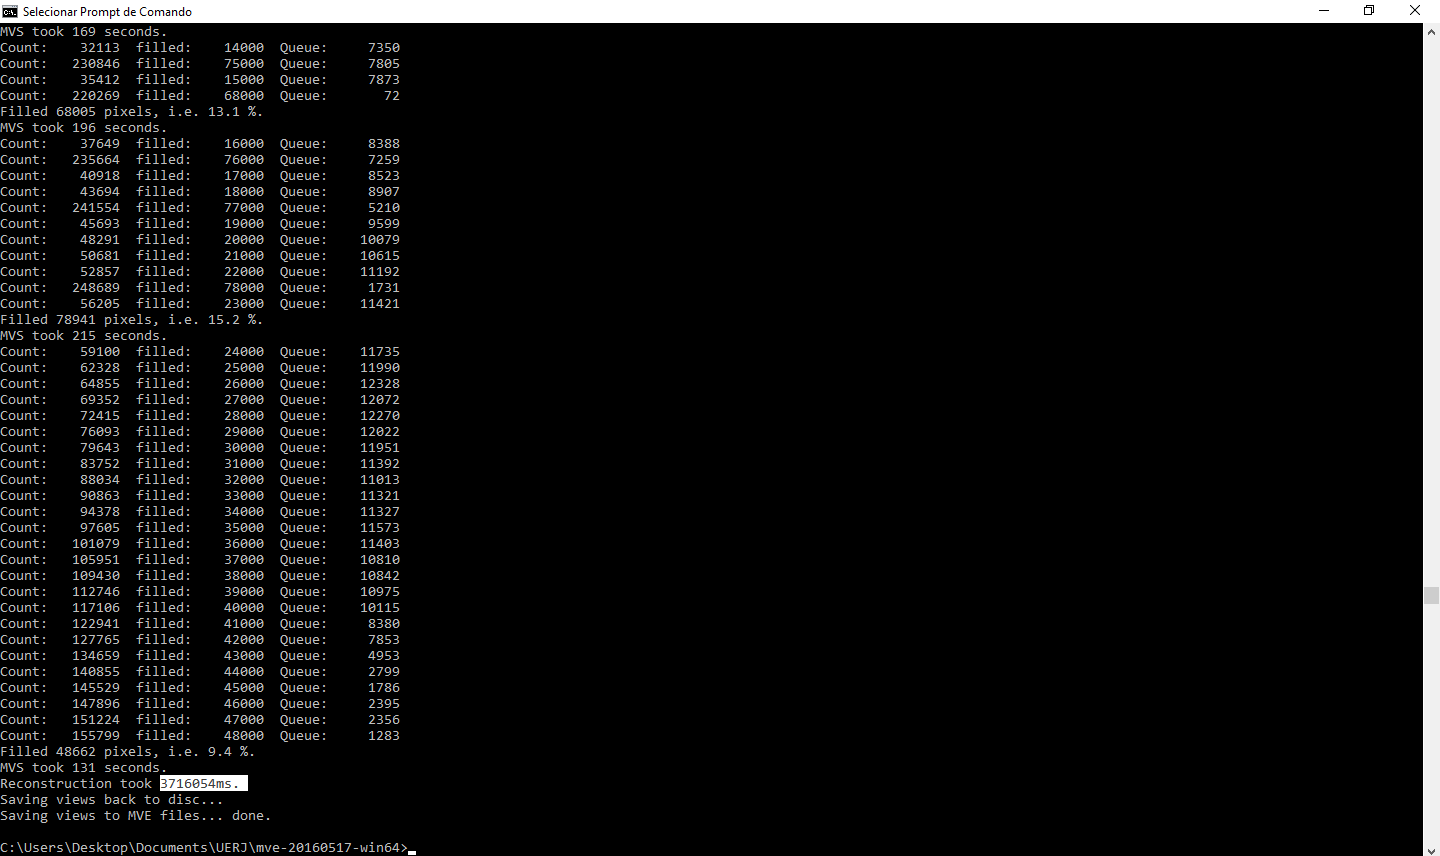
\includegraphics[width=0.5\linewidth]{figs/galinhadmreconmve.png}
	\caption{%
	Tempo da etapa {\it dmrecon} do MVE
	%\cite{Cui:Theobalt:etal:PAMI2013,Pajdla:etal:ICCV2011}.
	}\label{fig:dmrecon1}
\end{figure}

\begin{figure}[!h]
	\centering
	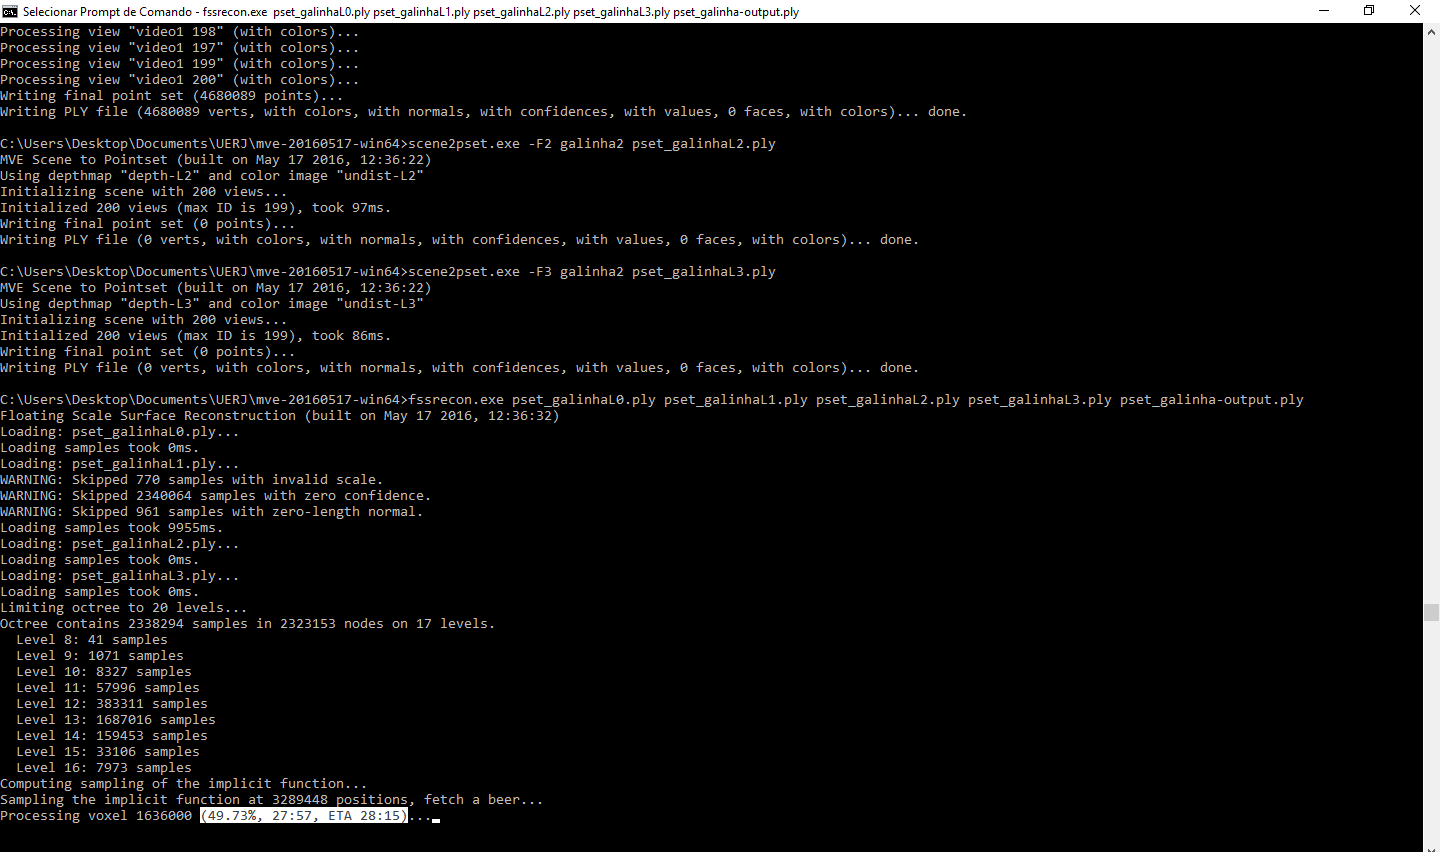
\includegraphics[width=0.5\linewidth]{figs/mvefssrecongalinha.png}
	\caption{%
	Tempo da etapa {\it fssrecon} do MVE
	%\cite{Cui:Theobalt:etal:PAMI2013,Pajdla:etal:ICCV2011}.
	}\label{fig:fssrecon}
\end{figure}

\begin{figure}[!h]
	\centering
	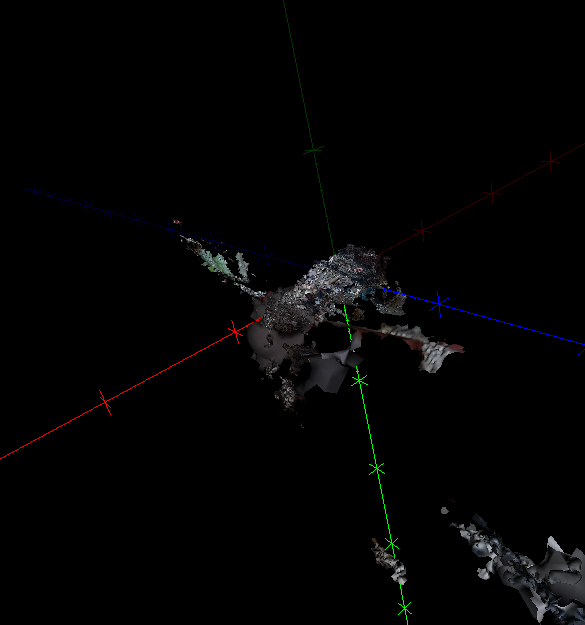
\includegraphics[width=0.5\linewidth]{figs/galinhadmr.png}
	\caption{%
	Resultado da etapa {\it fssrecon} do MVE
	%\cite{Cui:Theobalt:etal:PAMI2013,Pajdla:etal:ICCV2011}.
	}\label{fig:galinhaFssr}
\end{figure}

\begin{figure}[!h]
	\centering
	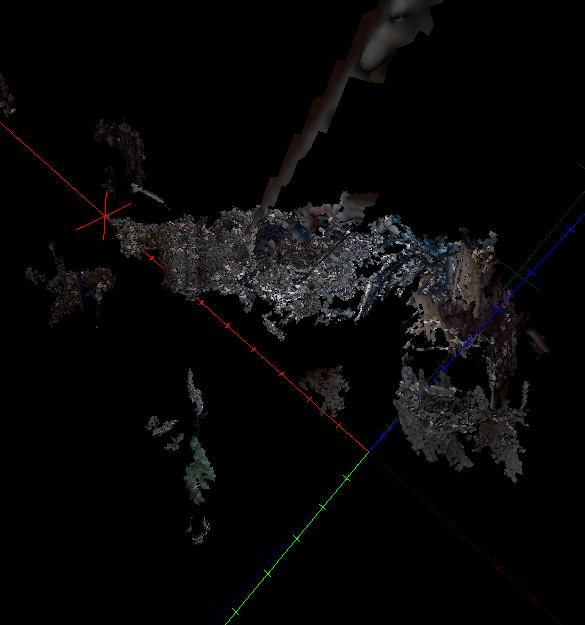
\includegraphics[width=0.5\linewidth]{figs/galinhameshclean.png}
	\caption{%
	Resultado da etapa {\it meshclean}, da etapa anterior \ref{fig:galinhaFssr}
	%\cite{Cui:Theobalt:etal:PAMI2013,Pajdla:etal:ICCV2011}.
	}\label{fig:galinhaMeshClean}
\end{figure}

A etapa de {\it scene2pset} demorou cerca de 20 segundos (total). Porém percebemos que a reconstrução não foi satisfatória, o {\it software} se confundiu, e não conseguiu obter os parâmetros corretos das câmeras utilizadas. A partir disso, o erro se propagou e gerou essa reconstrução acima \ref{fig:galinhaFssr} e \ref{fig:galinhaMeshClean}.

Rodamos também, com as 224 fotos, só foi possível executar o passo {\it sfmrecon} \ref{fig:galinhaSfM224}, pois o MVE não conseguiu rodar o comando {\it dmrecon} por algum motivo, e não gerou nenhum resultado para a continuação do algoritmo \ref{fig:galinhaDMR224}.

\begin{figure}[!h]
	\centering
	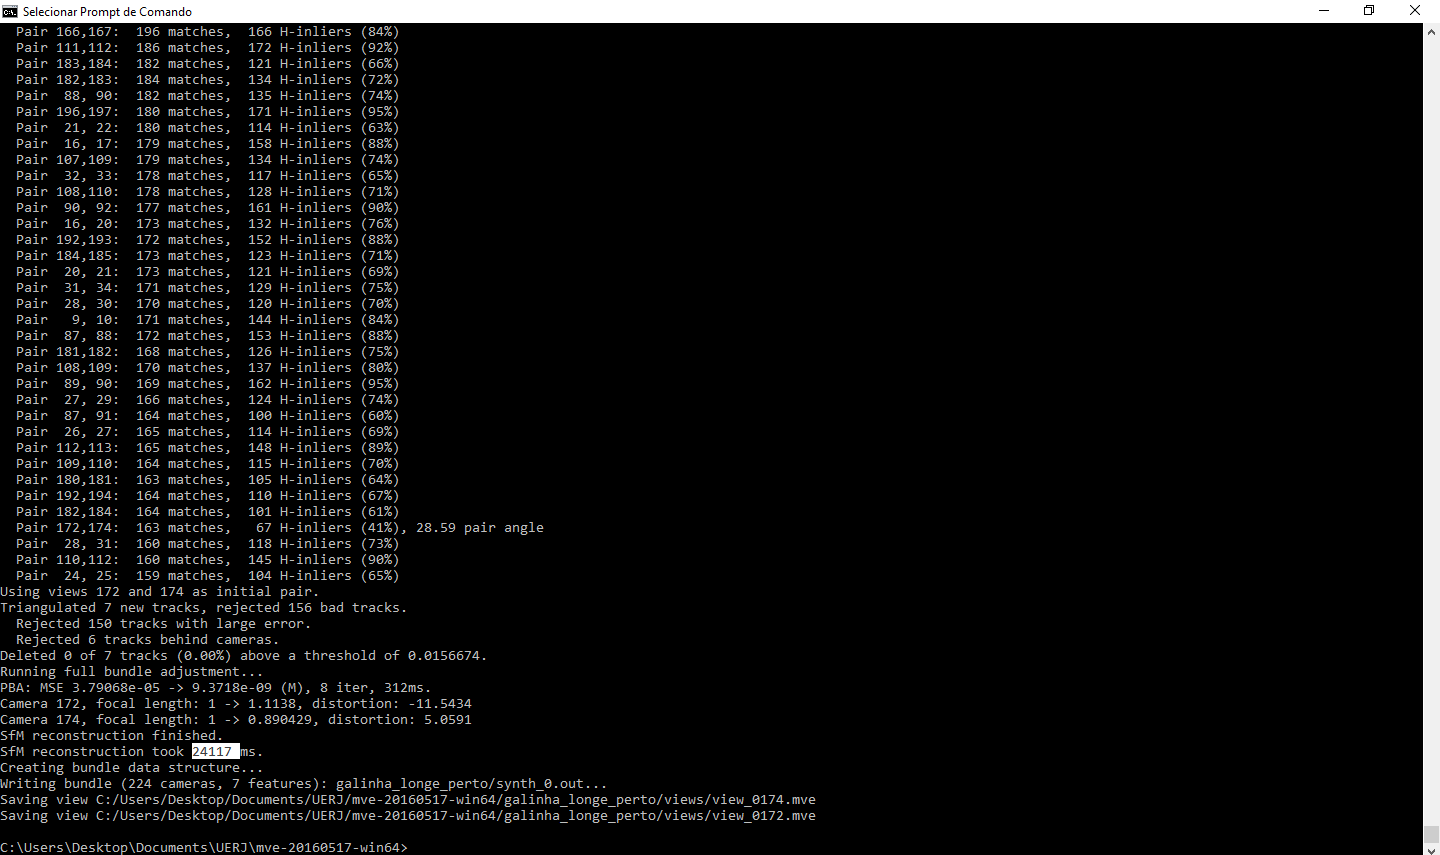
\includegraphics[width=0.5\linewidth]{figs/mvesfmrecongalinhapertolonge.png}
	\caption{%
	Resultado da etapa {\it sfmrecon}, com todas as imagens
	%\cite{Cui:Theobalt:etal:PAMI2013,Pajdla:etal:ICCV2011}.
	}\label{fig:galinhaSfM224}
\end{figure}

\begin{figure}[!h]
	\centering
	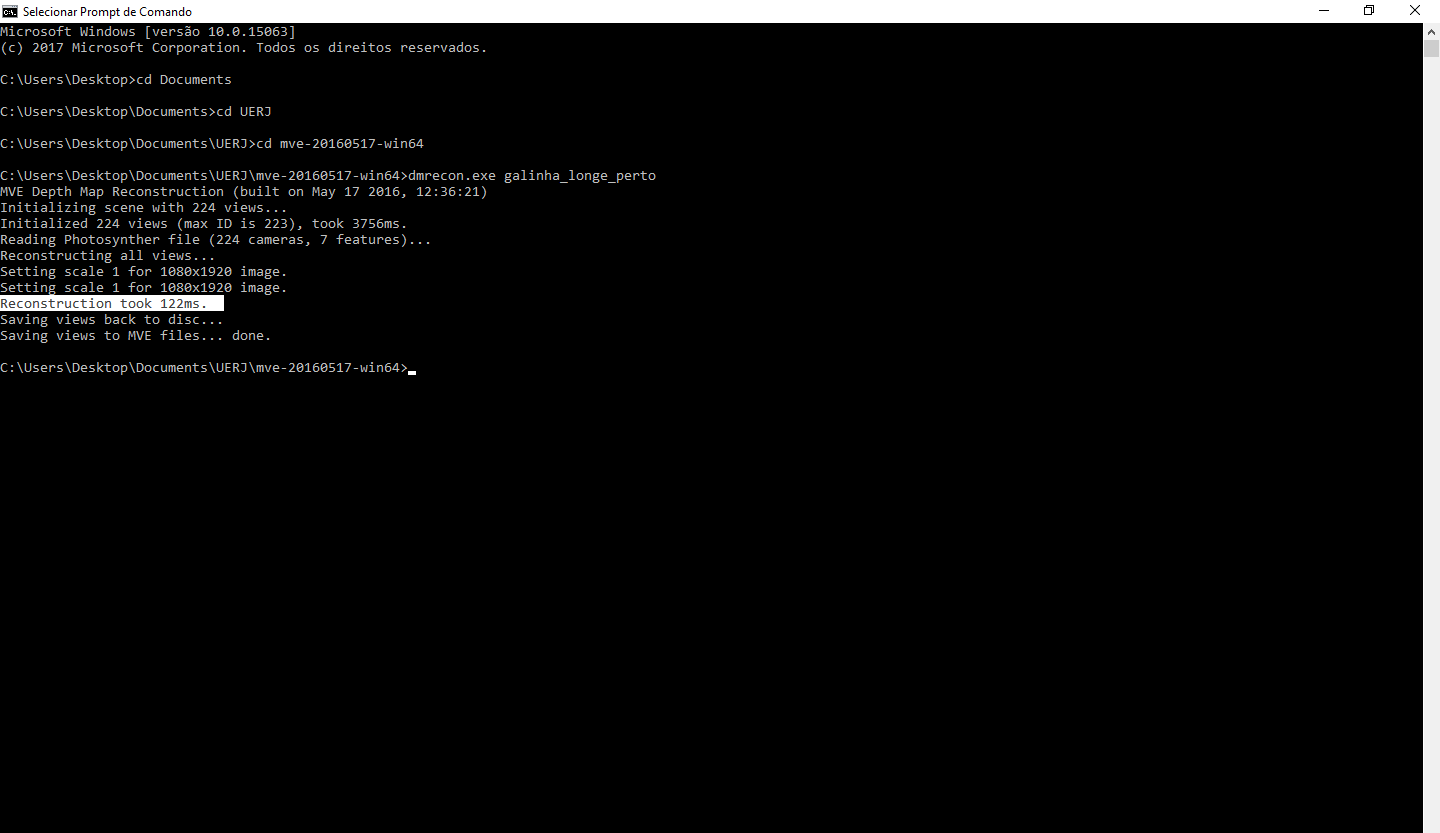
\includegraphics[width=0.5\linewidth]{figs/mvedmrecongalinhapertolonge.png}
	\caption{%
	Resultado da etapa {\it dmrecon}, com todas as imagens
	%\cite{Cui:Theobalt:etal:PAMI2013,Pajdla:etal:ICCV2011}.
	}\label{fig:galinhaDMR224}
\end{figure}
